% Options for packages loaded elsewhere
\PassOptionsToPackage{unicode}{hyperref}
\PassOptionsToPackage{hyphens}{url}
\PassOptionsToPackage{dvipsnames,svgnames,x11names}{xcolor}
\documentclass[
  10pt,
  fontset=fandol]{ctexart}
\usepackage{xcolor}
\usepackage[margin=16mm]{geometry}
\usepackage{amsmath,amssymb}
\setcounter{secnumdepth}{-\maxdimen} % remove section numbering
\usepackage{iftex}
\ifPDFTeX
  \usepackage[T1]{fontenc}
  \usepackage[utf8]{inputenc}
  \usepackage{textcomp} % provide euro and other symbols
\else % if luatex or xetex
  \usepackage{unicode-math} % this also loads fontspec
  \defaultfontfeatures{Scale=MatchLowercase}
  \defaultfontfeatures[\rmfamily]{Ligatures=TeX,Scale=1}
\fi
\usepackage{lmodern}
\ifPDFTeX\else
  % xetex/luatex font selection
\fi
% Use upquote if available, for straight quotes in verbatim environments
\IfFileExists{upquote.sty}{\usepackage{upquote}}{}
\IfFileExists{microtype.sty}{% use microtype if available
  \usepackage[]{microtype}
  \UseMicrotypeSet[protrusion]{basicmath} % disable protrusion for tt fonts
}{}
\makeatletter
\@ifundefined{KOMAClassName}{% if non-KOMA class
  \IfFileExists{parskip.sty}{%
    \usepackage{parskip}
  }{% else
    \setlength{\parindent}{0pt}
    \setlength{\parskip}{6pt plus 2pt minus 1pt}}
}{% if KOMA class
  \KOMAoptions{parskip=half}}
\makeatother
\usepackage{longtable,booktabs,array}
\newcounter{none} % for unnumbered tables
\usepackage{calc} % for calculating minipage widths
% Correct order of tables after \paragraph or \subparagraph
\usepackage{etoolbox}
\makeatletter
\patchcmd\longtable{\par}{\if@noskipsec\mbox{}\fi\par}{}{}
\makeatother
% Allow footnotes in longtable head/foot
\IfFileExists{footnotehyper.sty}{\usepackage{footnotehyper}}{\usepackage{footnote}}
\makesavenoteenv{longtable}
\usepackage{graphicx}
\makeatletter
\newsavebox\pandoc@box
\newcommand*\pandocbounded[1]{% scales image to fit in text height/width
  \sbox\pandoc@box{#1}%
  \Gscale@div\@tempa{\textheight}{\dimexpr\ht\pandoc@box+\dp\pandoc@box\relax}%
  \Gscale@div\@tempb{\linewidth}{\wd\pandoc@box}%
  \ifdim\@tempb\p@<\@tempa\p@\let\@tempa\@tempb\fi% select the smaller of both
  \ifdim\@tempa\p@<\p@\scalebox{\@tempa}{\usebox\pandoc@box}%
  \else\usebox{\pandoc@box}%
  \fi%
}
% Set default figure placement to htbp
\def\fps@figure{htbp}
\makeatother
\setlength{\emergencystretch}{3em} % prevent overfull lines
\providecommand{\tightlist}{%
  \setlength{\itemsep}{0pt}\setlength{\parskip}{0pt}}
\usepackage{amsmath,amssymb,mathtools,needspace}
\xeCJKDeclareCharClass{CJK}{"2032,"0400->"04FF,"2160->"216B,"2460->"2473,"25A0,"25C7,"25CB,"25CF}
\IfFontExistsTF{Arial Unicode MS}{\xeCJKsetup{AutoFallBack=true}\setCJKfallbackfamilyfont{\CJKrmdefault}{Arial Unicode MS}}{}
\setcounter{secnumdepth}{0}
\setlength{\emergencystretch}{2em}
\allowdisplaybreaks
\usepackage{bookmark}
\IfFileExists{xurl.sty}{\usepackage{xurl}}{} % add URL line breaks if available
\urlstyle{same}
\hypersetup{
  pdftitle={叠加计算},
  colorlinks=true,
  linkcolor={Maroon},
  filecolor={Maroon},
  citecolor={Blue},
  urlcolor={Blue},
  pdfcreator={LaTeX via pandoc}}

\title{叠加计算}
\author{}
\date{}

\begin{document}
\maketitle

\subsection{11.2　叠加计算}\label{ux53e0ux52a0ux8ba1ux7b97}

叠加计算是一类最简单、最基本的计算模型。本章所研究的叠加计算包括数列求和

\[
S=\sum_{i=0}^{N-1}a_i
\tag{11.2.1}
\]

与多项式求值

\[
P=\sum_{i=0}^{N-1}a_i x^i.
\tag{11.2.2}
\]

上述两种叠加计算模型之间有着紧密的联系。事实上，和式（11.2.1）是式（11.2.2）取 \(x=1\) 的具体情形。

在着手具体设计算法之前，首先引进问题的规模的概念。所谓规模是用来刻画问题``大小''的某个正整数。譬如，上述叠加计算问题的规模均可定为它们的项数 \(N\)。

不言而喻，并行计算所要求解的问题，其重要特点是规模很大，即为大规模或超大规模的科学计算。为简化叙述，今后将假定计算问题的规模 \(N\) 为 2 的幂，即

\[
N=2^n,
\]

式中，\(n=\log_2 N\) 是正整数。这种限制通常是非实质性的，譬如，对于上述两种叠加计算，只要适当地补充几个零系数 \(a_i\)，总可以将规模 \(N\) 扩充为 \(N=2^n\) 的形式。后文将会看到，这种扩充对于算法运行时间的影响几乎可以忽略不计。本章所考察的其他计算问题也可作类似的处理。

\subsubsection{11.2.1　倍增技术}\label{ux500dux589eux6280ux672f}

有些学者认为，倍增技术是设计同步并行算法的一项基本技术。这项设计技术反

\href{../../source-images/pdf-279.jpeg}{原页图像}

复地将计算问题分裂成具有同等规模的两个子问题。在问题逐步分裂的过程中，子问题的个数是逐步倍增的，倍增法因此而得名。

倍增法的设计基于这样的考虑，如果将各个子问题适当地映射到多台处理机上，即可实现计算过程的并行化。

现在就用简单的数列求和问题（11.2.1）考察倍增技术的设计原理和设计方法。为此，引进和式

\[
S(i,j)=\sum_{k=j}^{i}a_k.
\]

显然，问题（11.2.1）的已给数据与所求结果均可用这种和式来表达：

\[
\begin{gathered}
a_i=S(i,i),\quad i=0,1,\cdots,N-1;\\
S=S(N-1,0).
\end{gathered}
\]

倍增法的设计过程含分裂与合成两个环节。分裂过程将所给和式 \(S(N-1,0)\) 逐步``一分为二''，从而拆成若干个子和式。这种分裂过程的特点是，子和式的个数是逐步倍增的。

\[
\begin{aligned}
S(N-1,0)
&=S\left(N-1,\frac{N}{2}\right)+S\left(\frac{N}{2}-1,0\right)\\
&=S\left(N-1,\frac{3}{4}N\right)+S\left(\frac{3}{4}N-1,\frac{N}{2}\right)+S\left(\frac{N}{2}-1,\frac{N}{4}\right)+S\left(\frac{N}{4}-1,0\right)\\
&=\cdots.
\end{aligned}
\]

由于在和式二分的上述过程中，每个子和式的项数逐次减半，因而最终可拆成每段仅含两项的最简形式

\[
S(N-1,0)=S(N-1,N-2)+S(N-3,N-4)+\cdots+S(1,0).
\]

图 11.1 取 \(N=8\) 自顶向下地描述了倍增法的分裂过程。

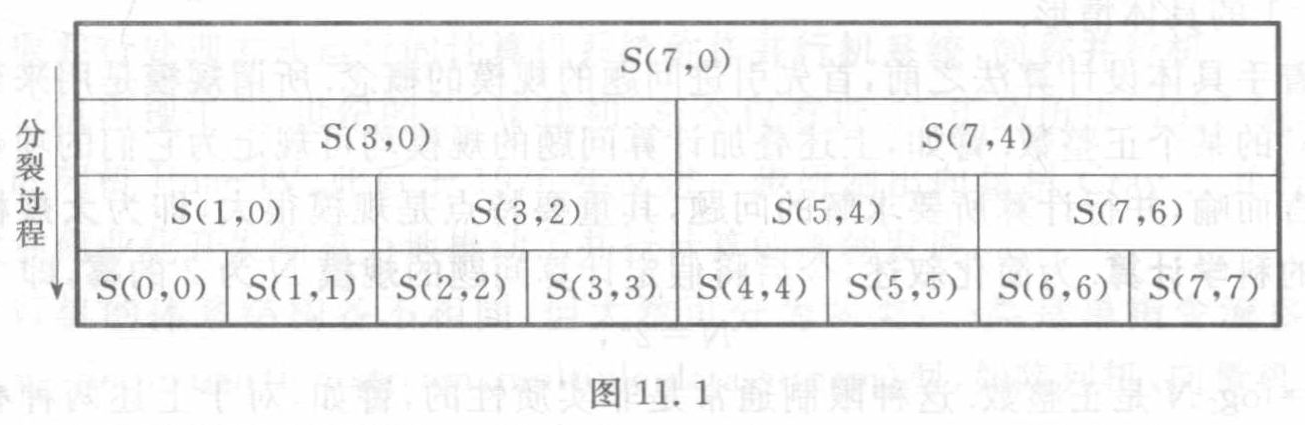
\includegraphics[width=0.85\linewidth,height=\textheight,keepaspectratio,alt={图 11.1（原图裁切）}]{../assets/ch11/figure-11-1.png}

图 11.1　原图的``分裂过程''箭头自上向下。各层由左至右的符号标签为：

{\def\LTcaptype{none} % do not increment counter
\begin{longtable}[]{@{}
  >{\raggedright\arraybackslash}p{(\linewidth - 2\tabcolsep) * \real{0.5000}}
  >{\raggedright\arraybackslash}p{(\linewidth - 2\tabcolsep) * \real{0.5000}}@{}}
\toprule\noalign{}
\begin{minipage}[b]{\linewidth}\raggedright
层次（由上至下）
\end{minipage} & \begin{minipage}[b]{\linewidth}\raggedright
原图中的子和式
\end{minipage} \\
\midrule\noalign{}
\endhead
\bottomrule\noalign{}
\endlastfoot
1 & \(S(7,0)\) \\
2 & \(S(3,0)\)，\(S(7,4)\) \\
3 & \(S(1,0)\)，\(S(3,2)\)，\(S(5,4)\)，\(S(7,6)\) \\
4 & \(S(0,0)\)，\(S(1,1)\)，\(S(2,2)\)，\(S(3,3)\)，\(S(4,4)\)，\(S(5,5)\)，\(S(6,6)\)，\(S(7,7)\) \\
\end{longtable}
}

每个上层区间对应下层相邻的两个子区间。（本段及上表为原图标签与结构的文字转录。）

将所给和式拆成若干个子和式后，可将这些子和式分配给各台处理机去并行计算。问题在于，基于这些子和式的计算，如何得出所求的结果呢？

倍增法的合成过程是将所拆出的各个子和式的值再逐步``合二为一''，最后归并出所给和式的值。这种归并过程的特点是数据量逐次减半。图 11.2 自底向上地描述了倍增法的合成过程。

\href{../../source-images/pdf-280.jpeg}{原页图像}

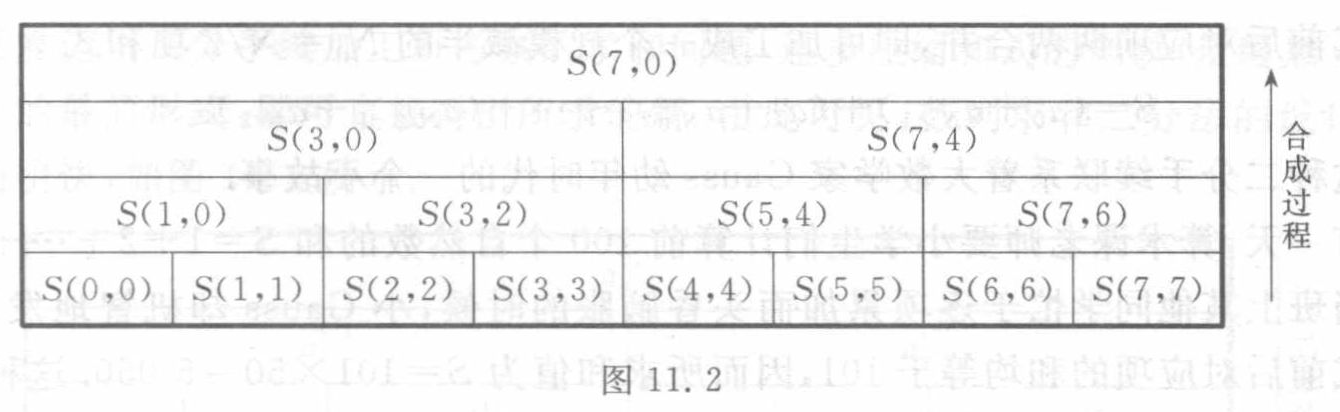
\includegraphics[width=0.85\linewidth,height=\textheight,keepaspectratio,alt={图 11.2（原图裁切）}]{../assets/ch11/figure-11-2.png}

图 11.2　原图``合成过程''箭头自下向上。各层从左至右的符号标签为：

{\def\LTcaptype{none} % do not increment counter
\begin{longtable}[]{@{}
  >{\raggedright\arraybackslash}p{(\linewidth - 2\tabcolsep) * \real{0.5000}}
  >{\raggedright\arraybackslash}p{(\linewidth - 2\tabcolsep) * \real{0.5000}}@{}}
\toprule\noalign{}
\begin{minipage}[b]{\linewidth}\raggedright
层次（由上至下）
\end{minipage} & \begin{minipage}[b]{\linewidth}\raggedright
原图中的子和式
\end{minipage} \\
\midrule\noalign{}
\endhead
\bottomrule\noalign{}
\endlastfoot
1 & \(S(7,0)\) \\
2 & \(S(3,0)\)，\(S(7,4)\) \\
3 & \(S(1,0)\)，\(S(3,2)\)，\(S(5,4)\)，\(S(7,6)\) \\
4 & \(S(0,0)\)，\(S(1,1)\)，\(S(2,2)\)，\(S(3,3)\)，\(S(4,4)\)，\(S(5,5)\)，\(S(6,6)\)，\(S(7,7)\) \\
\end{longtable}
}

每层中相邻的两个子区间向上合成为一个区间。（本段及上表为原图标签与结构的文字转录。）

现在列出倍增法的算法步骤（图 11.2）。

倍增法的第 1 步是利用所给的 \(N\) 个数据（它们均可视为一项和式）\(a_i=S(i,i)\) 求出 2 项和式的值，而得出 \(N_1=N/2\) 个中间结果：

\[
S(2i+1,2i)=S(2i+1,2i+1)+S(2i,2i),\quad i=0,1,\cdots,N_1-1.
\]

第 2 步再用两项和式求出 4 项和式的值，而有 \(N_2=N/4\) 个中间结果：

\[
S(4i+3,4i)=S(4i+3,4i+2)+S(4i+1,4i),\quad i=0,1,\cdots,N_2-1.
\]

保持和式项数逐步倍增，而数据量则为逐次减半这个特征，其第 \(k\) 步所承担的工作是，用 \(2^{k-1}\) 项和式求出 \(2^k\) 项和式的值，从而得出 \(N_k=N/2^k\) 个中间结果：

\[
\begin{gathered}
S(2^ki+2^k-1,2^ki)=S(2^ki+2^k-1,2^ki+2^{k-1})+S(2^ki+2^{k-1}-1,2^ki),\\
i=0,1,\cdots,N_k-1.
\end{gathered}
\tag{11.2.3}
\]

如此做 \(n=\log_2 N\) 步即可得出所求的和值：

\[
S(N-1,0)=S(N-1,N_1)+S(N_1-1,0).
\]

综上所述，数列求和（11.2.1）的倍增法可表述为算法 11.1。

\textbf{算法 11.1}　对 \(k=1,2,\cdots\) 直到 \(n=\log_2 N\) 执行算式（11.2.3），则所求的和值为 \(S=S(N-1,0)\)。

倍增法的分裂过程是反复将和式一分为二，在这一过程中，子和式的个数是逐步倍增的；与此相反，其合成过程是反复将数据合二为一，在合成过程中，数据量则为逐次减半。正是由于倍增法的分裂过程与合成过程相对峙，这种技术不便于实际运用。

\subsubsection{11.2.2　二分手续}\label{ux4e8cux5206ux624bux7eed}

为使并行算法设计的原理与方法简单而和谐，这里推荐一种设计技术------二分技术。

\textbf{二分技术的设计原理是，反复地将所给计算问题加工成规模减半的同类问题，直到规模足够小（通常当规模为 1）时直接得出问题的解。}

\textbf{需要强调的是，与倍增技术不同，二分技术不是着眼于问题的分裂，而是立足于问题的加工。今后所说的二分手续，是指将问题规模减半的加工手续。}

譬如，对于 \(N\) 项和式

\[
S=\sum_{i=0}^{N-1}a_i,
\]

\href{../../source-images/pdf-281.jpeg}{原页图像}

若将其前后对应项两两合并，即可加工成一个规模减半的 \(N_1=N/2\) 项和式

\[
S=(a_0+a_{N-1})+(a_1+a_{N-2})+\cdots+(a_{N/2-1}+a_{N/2}).
\]

这种二分手续联系着大数学家 Gauss 幼年时代的一个小故事。

有一天，算术课老师要小学生们计算前 100 个自然数的和 \(S=1+2+\cdots+99+100\)。当班上其他同学忙于逐项累加而头昏脑胀的时候，小 Gauss 却机智地发现，所给和式前后对应项的和均等于 101，因而所求和值为 \(S=101\times50=5\,050\)。这种简捷的快速算法可以视作二分手续的巧妙应用。

\subsubsection{11.2.3　数列求和的二分法}\label{ux6570ux5217ux6c42ux548cux7684ux4e8cux5206ux6cd5}

再考察所给和式（10.2.1），容易看出，如果将其奇偶项两两合并，即可使其规模变成 \(N_1=N/2\)，即

\[
S=\sum_{i=0}^{N_1-1}(a_{2i}+a_{2i+1})=\sum_{i=0}^{N_1-1}a_i^{(1)}.
\]

为此，所要施行的运算手续是

\[
a_i^{(1)}=a_{2i}+a_{2i+1},\quad i=0,1,\cdots,N_1-1.
\]

注意到这样加工出的求和问题

\[
S=\sum_{i=0}^{N_1-1}a_i^{(1)}
\]

与所给问题（10.2.1）属于同一类型，所不同的只是规模缩减了一半，因此上述加工手续是一种二分手续。

反复施行这种二分手续，二分 \(k\) 次后和式的项数压缩成 \(N_k=N/2^k\)，即

\[
S=\sum_{i=0}^{N_k-1}a_i^{(k)},
\]

式中

\[
a_i^{(k)}=a_{2i}^{(k-1)}+a_{2i+1}^{(k-1)},\quad i=0,1,\cdots,N_k-1.
\tag{11.2.4}
\]

这样二分 \(n=\log_2 N\) 次后，所给和式最终退化为一项，从而直接得出所求的和值 \(S\)。于是有数列求和的二分算法 11.2。

\textbf{算法 11.2}　对 \(k=1,2,\cdots\) 直到 \(n=\log_2 N\) 执行算式（11.2.4），结果有

\[
S=a_0^{(n)}.
\]

这一算法显然可以向量化。事实上，算式（11.2.4）可以表为向量形式：

\[
\begin{pmatrix}
a_0^{(k)}\\
a_1^{(k)}\\
\vdots\\
a_{N_k-1}^{(k)}
\end{pmatrix}
=
\begin{pmatrix}
a_0^{(k-1)}\\
a_2^{(k-1)}\\
\vdots\\
a_{N_{k-1}-2}^{(k-1)}
\end{pmatrix}
+
\begin{pmatrix}
a_1^{(k-1)}\\
a_3^{(k-1)}\\
\vdots\\
a_{N_{k-1}-1}^{(k-1)}
\end{pmatrix}.
\]

\begin{quote}
校注（agent 补充，CH11-E001）：本页两处回引均印作``（10.2.1）''，已照录；从本节的数列求和定义及上下文判断，应回引本章的式（11.2.1）。这是原书交叉引用疑误，不是 OCR 改写。
\end{quote}

\href{../../source-images/pdf-282.jpeg}{原页图像}

反复运用二分手续加工所考察的求和问题，逐步压缩和式的规模，最终加工成规模为 1 的最简形式，即可直接得出所求的解。由此可见，数列求和二分法的设计过程简洁而明快，如图 11.3 所示。

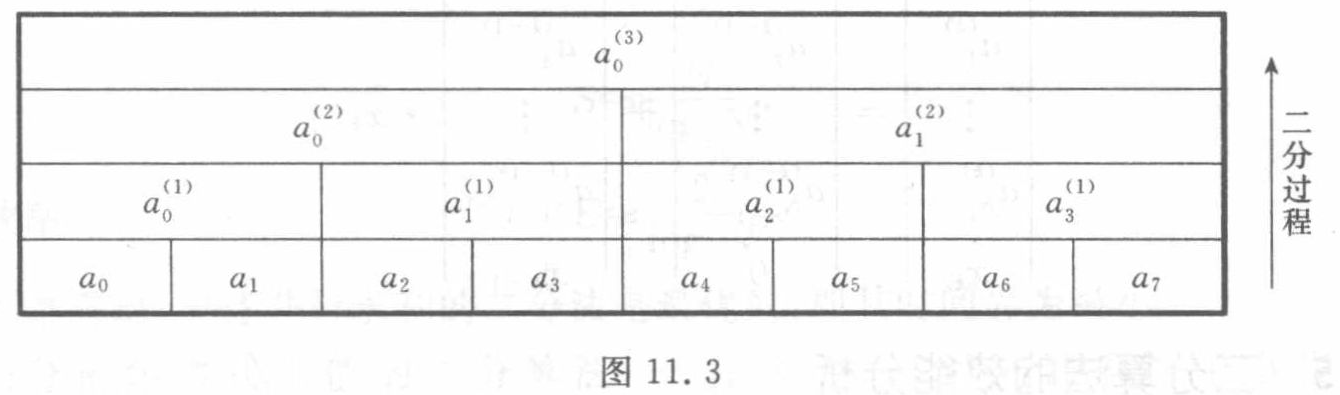
\includegraphics[width=0.85\linewidth,height=\textheight,keepaspectratio,alt={图 11.3（原图裁切）}]{../assets/ch11/figure-11-3.png}

图 11.3　原图``二分过程''箭头自下向上。各层从左至右的符号标签为：

{\def\LTcaptype{none} % do not increment counter
\begin{longtable}[]{@{}ll@{}}
\toprule\noalign{}
层次（由下至上） & 原图中的数据 \\
\midrule\noalign{}
\endhead
\bottomrule\noalign{}
\endlastfoot
初始层 & \(a_0\)，\(a_1\)，\(a_2\)，\(a_3\)，\(a_4\)，\(a_5\)，\(a_6\)，\(a_7\) \\
第 1 次二分 & \(a_0^{(1)}\)，\(a_1^{(1)}\)，\(a_2^{(1)}\)，\(a_3^{(1)}\) \\
第 2 次二分 & \(a_0^{(2)}\)，\(a_1^{(2)}\) \\
第 3 次二分 & \(a_0^{(3)}\) \\
\end{longtable}
}

每次将相邻两格合为上层的一格。（本段及上表为原图标签与结构的文字转录。）

应当指出的是，上面提供的两个算法------算法 11.1 和算法 11.2，尽管思路不同，繁简互异，但却是殊途同归。事实上，式（11.2.4）与式（11.2.3）得出的是同样的结果：

\[
a_i^{(k)}=S(2^ki+2^k-1,2^ki).
\]

\subsubsection{11.2.4　多项式求值的二分法}\label{ux591aux9879ux5f0fux6c42ux503cux7684ux4e8cux5206ux6cd5}

进一步讨论多项式求值问题。仿照数列求和的做法，将所给多项式（11.2.2）的奇偶项两两合并，得

\[
P=\sum_{i=0}^{N_1-1}(a_{2i}+a_{2i+1}x)x^{2i}.
\]

若令

\[
\begin{cases}
a_i^{(1)}=a_{2i}+a_{2i+1}x,\quad i=0,1,\cdots,N_1-1,\\
x_1=x^2,
\end{cases}
\]

则有

\[
P=\sum_{i=0}^{N_1-1}a_i^{(1)}x_1^i.
\]

这样加工得出的是一个以 \(x_1\) 为变元的多项式，它与所给多项式（11.2.2）的类型相同，只是规模压缩了一半，因此上述手续是一项二分手续。

重复这种手续，二分 \(k\) 次后所给多项式被加工成

\[
P=\sum_{i=0}^{N_k-1}a_i^{(k)}x_k^i,
\]

这里

\[
\begin{cases}
a_i^{(k)}=a_{2i}^{(k-1)}+a_{2i+1}^{(k-1)}x_{k-1},\quad i=0,1,\cdots,N_k-1,\\
x_k=x_{k-1}^2.
\end{cases}
\tag{11.2.5}
\]

这样二分 \(n=\log_2 N\) 次，最终得出的系数 \(a_0^{(n)}\) 即为所求多项式的值 \(P\)。于是，多项式求值问题（11.2.2）有多项式求值的二分算法 11.3。

\textbf{算法 11.3}　对 \(k=1,2,\cdots\) 直到 \(n=\log_2 N\) 执行算式（11.2.5），结果有

\href{../../source-images/pdf-283.jpeg}{原页图像}

\[
P=a_0^{(n)}.
\]

上述算法同样可以向量化，事实上，算式（11.2.5）可表为向量化形式：

\[
\begin{pmatrix}
a_0^{(k)}\\
a_1^{(k)}\\
\vdots\\
a_{N_k-1}^{(k)}\\
x_k
\end{pmatrix}
=
\begin{pmatrix}
a_0^{(k-1)}\\
a_2^{(k-1)}\\
\vdots\\
a_{N_{k-1}-2}^{(k-1)}\\
0
\end{pmatrix}
+
\begin{pmatrix}
a_1^{(k-1)}\\
a_3^{(k-1)}\\
\vdots\\
a_{N_{k-1}-1}^{(k-1)}\\
x_{k-1}
\end{pmatrix}\cdot x_{k-1}.
\]

\subsubsection{11.2.5　二分算法的效能分析}\label{ux4e8cux5206ux7b97ux6cd5ux7684ux6548ux80fdux5206ux6790}

评价一种并行算法，人们首先关心的是它的算法复杂性，即算法的运行时间（时间复杂性）与所要提供的处理机台数（空间复杂性）。并行算法设计的基本思想是用增加处理机台数的办法来换取算法运行时间的节省。处理机台数充分多时的最少运行时间称作算法的时间界，而算法的运行时间达到时间界时所需提供的（最少的）处理机台数则称作处理机台数界。

为简化分析，今后将假定每台处理机的算术运算（无论是加减还是乘除）的操作时间相同，均取单位时间。这样，在估算算法的运行时间时，只要针对各并行步骤统计运算次数即可。

对于所考察的某个并行算法，记 \(T^*\) 为算法的时间界，\(P^*\) 为处理机台数界，另记 \(T_1\) 为串行算法的运行时间，将

\[
S=\frac{T_1}{T^*}
\]

称作该并行算法的加速比，而将

\[
E=\frac{T_1}{P^*T^*}
\]

称作其效率。

加速比与效率是评估一种并行算法的``得''与``失''的两项重要指标。加速比 \(S\) 表示该并行算法在运行时间方面的节省；注意到 \(P^*T^*\) 表示并行算法的总计算量，而 \(T_1\) 则表示串行算法的计算量，因而效率 \(E\) 刻画了该并行算法在计算量方面的损耗。

现在分析前述几种二分算法的时间界与处理机台数界。

首先考察数列求和的二分算法------算法 11.2。令式（11.2.4）的各个系数 \(a_i^{(k)}\) 并行计算，则其每一步含一次运算（加法），故其时间界为

\[
T^*=n=\log_2 N.
\]

然而，为使每个 \(a_i^{(k)}\) 能并行计算，第 \(k\) 步按式（11.2.4）需提供 \(N_k=N/2^k\) 台处理机，因此算法 11.2 的处理机台数界为

\href{../../source-images/pdf-284.jpeg}{原页图像}

\[
P^*=\max_{1\le k\le n}\frac{N}{2^k}=\frac{N}{2}.
\]

注意到数列求和问题（11.2.1）的串行算法的运行时间 \(T_1=N-1\)，算法 11.2 的加速比

\[
S\approx\frac{N}{\log_2 N},
\]

而其效率

\[
E\approx\frac{2}{\log_2 N}.
\]

不难看出，上述并行求和的二分法是最优的，即其时间界为最小。

再分析多项式求值的二分算法------算法 11.3。首先注意一个事实：算式（11.2.5）中的 \(x_k\) 可与 \(a_i^{(k)}\) 并行计算，为此只要将式 \(x_k=x_{k-1}^2\) 改写成

\[
x_k=0+x_{k-1}\cdot x_{k-1}
\]

的形式。这样，算法 11.3 的每一步需做 2 次运算（一次乘法与一次加法），因而其时间界为

\[
T^*=2\log_2 N.
\]

此外，为使 \(a_i^{(k)}\) 与 \(x_k\) 按式（11.2.5）并行计算，第 \(k\) 步需处理机 \(N/2^k\) 台，因此算法 11.3 的处理机台数界为

\[
P^*=\max_{1\le k\le n}\frac{N}{2^k}=\frac{N}{2}.
\]

注意到多项式求值的串行算法（秦九韶-Horner 算法）需做 \(T_1=2(N-1)\) 次运算，易知算法 11.3 的加速比及效率均与算法 11.2 相同，仍为

\[
S\approx\frac{N}{\log_2 N},\quad E\approx\frac{2}{\log_2 N}.
\]

\subsubsection{11.2.6　二分算法的基本特征}\label{ux4e8cux5206ux7b97ux6cd5ux7684ux57faux672cux7279ux5f81}

本小节从最简单的计算模型------叠加计算入手，考察并行计算的二分算法的基本特征。

在设计原理上，并行的二分算法与串行的递推算法，两者的设计过程都是计算模型不断演化的过程，其区别在于，串行递推算法的规模逐次减 1，而并行二分算法的规模则为逐次减半。例如，累加求和算法的加工过程为

\(N\) 项和式 \(\to\) \(N-1\) 项和式 \(\to\) \(N-2\) 项和式 \(\to\cdots\to\) 1 项和式，

而二分求和算法的加工过程是

\(N\) 项和式 \(\Rightarrow\) \(N/2\) 项和式 \(\Rightarrow\) \(N/4\) 项和式 \(\Rightarrow\cdots\Rightarrow\) 1 项和式。

可见，串行算法与并行算法的设计思想是一脉相承的，后者可以视作是前者的延伸与发展。

从算法的结构来看，并行的二分算法与串行递推算法均具有递归结构，即将复杂

\begin{quote}
校注（agent 补充，CH11-E002）：多项式算法的处理机计数按原书照录。上一页的向量形式同时更新 \(N_k\) 个系数及 \(x_k\)，共有 \(N_k+1\) 个分量；在原书所述每个分量完全同步执行一次乘法和一次加法的安排下，处理机数应计入计算 \(x_k\) 的额外一台。原书此处写 \(N/2^k\)，可能省略了常数项或依赖未说明的调度，属处理机台数界的疑误；未据此改动原式。
\end{quote}

\href{../../source-images/pdf-285.jpeg}{原页图像}

计算归结为简单计算的重复。譬如数列求和计算，是将多项求和归结为简单的二项求和的重复，而多项式求值是将高次式求值归结为简单的一次式求值的重复，等等。对串行算法这里所谓``重复''意味着循环，而并行算法所指的``重复''则综合采取串行与并行两种处理方式。

从算法效能的角度来看，串行算法与并行算法各有所长，前者拥有高效率，而后者则具有高速度。不过，并行算法的高速度是以处理机台数的增加为代价的。

\subsection{本节覆盖原页的校注记录}\label{ux672cux8282ux8986ux76d6ux539fux9875ux7684ux6821ux6ce8ux8bb0ux5f55}

下列记录按原页关联，含同页相邻小节的校注；计算时同时读取上文校注和完整原页。

\begin{itemize}
\tightlist
\item
  \texttt{CH11-E001}：原书 PDF 页 281
\item
  \texttt{CH11-E002}：原书 PDF 页 284
\end{itemize}

\end{document}
